%==============================================================================
% FAAT: Feature-Aligned Adaptive Triggers for Clean-Label Backdoor Attacks
% CVPR submission (review / double-blind). Template: cvpr-org/author-kit.
% Compile:  latexmk -pdf main
%==============================================================================
\documentclass[10pt,twocolumn,letterpaper]{article}

%%%%%%%%% PAPER TYPE  - pick ONE
\usepackage[review]{cvpr}       % REVIEW version (anonymous, line numbers)
% \usepackage{cvpr}             % CAMERA-READY version
% \usepackage[pagenumbers]{cvpr}% arXiv version with page numbers

% Extra packages + small macros (loaded BEFORE hyperref)
%% Additional packages and macros for the FAAT paper.
%% Loaded by main.tex before hyperref.

% --- pseudo-code ---
\usepackage{algorithm}
\usepackage{algorithmic}

% (architecture diagram F2 is rendered with matplotlib -> no tikz needed;
%  tikz pulls everyshi which clashes with cvpr.sty's inlined everyshi.)
\floatname{algorithm}{Algorithm}
\renewcommand{\algorithmicrequire}{\textbf{Input:}}
\renewcommand{\algorithmicensure}{\textbf{Output:}}

% --- tables / layout ---
\usepackage{multirow}
\usepackage{array}
\usepackage{cuted}     % strip environment (two-column teaser)
\usepackage{currfile}  % \currfilebase

% --- inline annotations (disable for final) ---
\newcommand{\red}[1]{{\color{red}#1}}
\newcommand{\todo}[1]{{\color{red}#1}}
\newcommand{\TODO}[1]{\textbf{\color{red}[TODO: #1]}}
% For camera-ready, uncomment to hide todos:
% \renewcommand{\TODO}[1]{}
% \renewcommand{\todo}[1]{#1}

% --- paper-specific macros ---
\newcommand{\faat}{FAAT}                         % our main method
\newcommand{\kst}{KST}                           % spectrum-flat trigger
\newcommand{\sdt}{SDT}                           % Stein trigger
\newcommand{\dglobal}{\delta_{\mathrm{g}}}       % global trigger
\newcommand{\dadapt}{\delta_{\mathrm{a}}}        % adaptive residual
\newcommand{\Lalign}{\mathcal{L}_{\mathrm{align}}}
\newcommand{\asr}{\mathrm{ASR}}                  % attack success rate
\newcommand{\ba}{\mathrm{BA}}                    % benign accuracy
\newcommand{\ours}{\textbf{Ours}}                % bold "Ours" in tables
\newcommand{\na}{\textendash}                    % placeholder for not-yet-filled cells
\newcommand{\secsub}[1]{\textsubscript{#1}}      % tiny subscript helper


\definecolor{cvprblue}{rgb}{0.21,0.49,0.74}
\usepackage[pagebackref,breaklinks,colorlinks,allcolors=cvprblue]{hyperref}

%%%%%%%%% PAPER METADATA
\def\paperID{*****}            % *** Enter the (anonymous) Paper ID here
\def\confName{CVPR}
\def\confYear{2026}            % bump to your target year (e.g. 2027)

%%%%%%%%% TITLE
\title{Feature-Aligned Adaptive Triggers for Effective\\
and Stealthy Clean-Label Backdoor Attacks}

%%%%%%%%% AUTHORS  (double-blind: keep anonymous for review)
\author{Anonymous Author(s)\\
Institution\\
{\tt\small anonymous@institution}
}

\begin{document}
\maketitle

% ---------- Teaser figure ----------
\begin{figure*}[t]
\centering
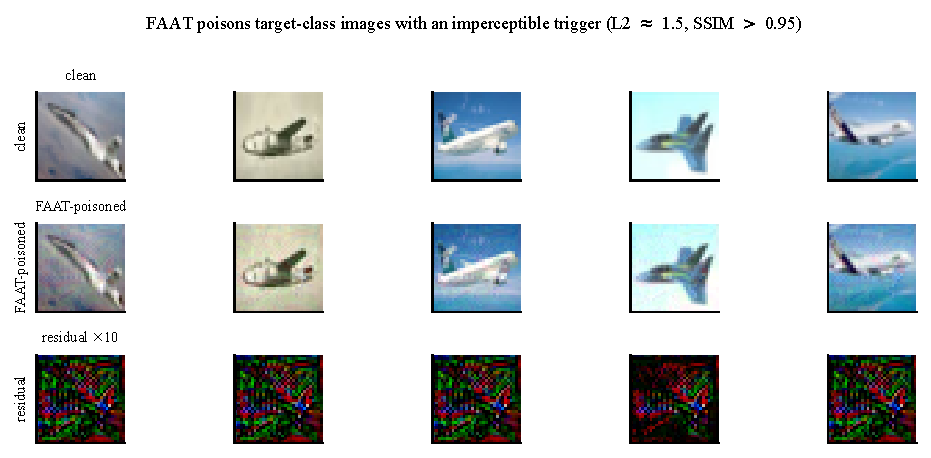
\includegraphics[width=0.92\linewidth]{floats/figures/f1_teaser.pdf}
\caption{\textbf{FAAT poisons target-class training images with an imperceptible
trigger.} Each poisoned sample carries a global direction~$\dglobal$ plus a
bounded per-sample adaptive residual~$\dadapt$ (shown amplified $\times$10 in the
bottom row). The perturbation is small ($\ell_2\!\approx\!1.5$, SSIM $>$ 0.95)
yet yields $\asr\!=\!93.6\%$ on CIFAR-10 while keeping benign accuracy intact,
and is not flagged by sample-filtering defenses.}
\label{fig:teaser}
\end{figure*}


% ---------- Abstract ----------
\begin{abstract}
Clean-label backdoor attacks are appealing because they leave poison-label
annotations untouched, yet current methods become unreliable when the victim
task is hard---many-class, low-poison-rate, or high-base-accuracy regimes where
a small, fixed trigger is diluted by the strong benign signal.
We present \textbf{FAAT} (Feature-Aligned Adaptive Trigger), a clean-label
attack composed of three generalized components: (i) a \emph{frozen global
direction} $\dglobal$ that supplies a strong, transferable backdoor signal;
(ii) a \emph{bounded adaptive residual} $\dadapt$ shaped in the DCT domain that
restores effectiveness while staying imperceptible; and (iii) a
\emph{feature-alignment loss} $\Lalign$ that pulls poisoned representations
toward the target class so sample-clustering defenses cannot isolate them.
FAAT is trained self-containedly, with no external pre-optimized noise.
On CIFAR-10, CIFAR-100 and Tiny-ImageNet, FAAT raises attack success rate
by $+3.9$ to $+51.9$ points over the strongest reproduced clean-label baseline,
with benign accuracy intact (SSIM $0.92$--$0.98$, $\ell_2\!\le\!1.5$ on natural
images), and is not flagged by Activation Clustering, Spectral Signatures,
STRIP or Fine-Pruning. As a complementary contribution we introduce \textbf{KST},
a trigger whose spectrum is \emph{structurally flat} (peak/median $\approx\!1.0$,
vs.\ $68.8$ for Narcissus), defeating frequency-domain defenses at ASR parity.
Finally, we treat GTSRB not as a fourth dataset but as a \emph{stress test of
overconfident victims} (BA$\approx\!100\%$): there, fixed, flat-spectrum and
adaptive triggers each reveal a distinct failure mode, exposing a fundamental
ASR--stealth trade-off that tightens as victim confidence grows.
\end{abstract}


% ---------- Body (restructured 2026-09-17: 6 top-level sections) ----------
%  1 Introduction                sections/01_intro.tex
%  2 Related Work                sections/02_related.tex
%  3 Method                      sections/03_method.tex
%      3.1 Problem Formulation and Threat Model
%      3.2 Overview of FAAT      <- Fig.2 framework figure
%      3.3 Global Trigger Generation
%      3.4 Sample-Adaptive Residual
%      3.5 Feature-Aligned Optimization
%      3.6 Poison Construction and Victim Training
%  4 Experiments                 sections/04_experiments.tex
%      4.1 Experimental Setup / 4.2 Main Results / 4.3 Defense Robustness
%      4.4 Ablation Study / 4.5 Stealth--Effectiveness Trade-off
%  5 Further Analysis            sections/05_analysis.tex
%      5.1 KST / 5.2 GTSRB stress test / 5.3 Discussion and Limitations
%  6 Conclusion                  sections/09_conclusion.tex
\section{Introduction}
\label{sec:intro}

Deep neural networks are known to be vulnerable to \emph{backdoor attacks}: an
adversary poisons a fraction of the training data so that the learned model
behaves normally on clean inputs but misclassifies any input bearing a trigger
to a target label~\cite{gu2017badnets}. Most early attacks
\emph{flip the label} of poisoned samples, which is easy to spot under visual
inspection. \textbf{Clean-label} attacks~\cite{turner2018labelconsist,chen2019blended}
are stealthier: poisoned samples keep their \emph{true} (target-class) label, so
the attack is invisible to label-level auditing. Their price is effectiveness:
without a label signal telling the model \emph{where} the trigger is, the model
must discover the trigger on its own, which requires either large triggers or
careful sample selection.

A recent line of work~\cite{generalcomponents2025} systematizes this with three
\emph{generalized components}---a quantization/blend trigger, a sample-selection
criterion, and a clean-label training protocol---and shows that the right
combination (e.g.\ a residual-squared selection) recovers competitive attack
success rates (ASR) on CIFAR-10. \textbf{However, the approach is brittle beyond
that comfort zone.} We reproduce these components faithfully and observe two
failure modes (Fig.~\ref{fig:main}): (1) on \emph{many-class / low-poison}
regimes (CIFAR-100 at $0.5\%$, Tiny-ImageNet at $0.25\%$) the strongest baseline
reaches only $\sim$44--85\% ASR; (2) on \emph{high-base-accuracy} tasks
(GTSRB, BA$\approx$100\%) the fixed trigger is diluted to $\le 34\%$ ASR---and
two of four baselines collapse to $0\%$. In all cases the benign task is so
easily learned that the tiny poison signal is washed out.

We argue the fix is to make the trigger \emph{adaptive and feature-aware} rather
than fixed. We propose \textbf{FAAT} (Feature-Aligned Adaptive Trigger), which
adds three components on top of the clean-label framework:
\begin{itemize}[leftmargin=*,topsep=2pt,itemsep=1pt]
  \item A \textbf{frozen global direction} $\dglobal$ (Narcissus-style~\cite{zeng2023narcissus})
        supplies a strong, transferable backdoor signal that is robust to benign dilution.
  \item A \textbf{bounded adaptive residual} $\dadapt$, optimized \emph{per poisoned
        image} in the DCT domain and clipped to a small $\ell_2$ budget, restores
        attack effectiveness without sacrificing imperceptibility.
  \item A \textbf{feature-alignment loss} $\Lalign$ pulls the representations of
        poisoned samples toward the target-class centroid, so that
        Activation-Clustering~\cite{chen2018activation} and
        Spectral-Signature~\cite{tran2018spectral} defenses cannot separate them
        from clean target-class samples.
\end{itemize}
All three are trained \emph{self-containedly}---FAAT does not depend on any
external pre-optimized noise, unlike Narcissus. Across CIFAR-10, CIFAR-100 and
Tiny-ImageNet, FAAT improves ASR by $+3.9$ to $+51.9$ points over the strongest
reproduced baseline (Tab.~\ref{tab:main}), preserves benign accuracy, stays
stealthy (SSIM $0.92$--$0.98$), and is not flagged by four sample-level defenses
(Tab.~\ref{tab:defense}). As a complementary contribution, \textbf{KST} is a
trigger variant whose DFT spectrum is \emph{structurally flat}
(peak/median $\approx\!1.0$ vs.\ $68.8$ for Narcissus), providing the first
clean-label trigger that defeats frequency-domain defenses at ASR parity
(Sec.~\ref{sec:kst}).

\paragraph{Contributions.} (1) FAAT, a self-contained clean-label backdoor with
a frozen global direction, a bounded DCT adaptive residual, and a
feature-alignment loss; (2) state-of-the-art clean-label ASR on three datasets,
especially on hard regimes where prior baselines collapse; (3) a systematic
defense evaluation showing FAAT evades sample-filtering defenses; (4) KST, a
flat-spectrum trigger that structurally evades frequency-domain
defenses.
         % 1
\section{Related Work}
\label{sec:related}

\paragraph{Backdoor attacks.}
BadNets~\cite{gu2017badnets} introduced pixel-patch triggers; subsequent work
made triggers imperceptible via blending~\cite{chen2019blended},
sinusoidal stripes~\cite{barni2020sig}, warping~\cite{nguyen2021wanet},
steganography~\cite{li2021ssba}, and quantization~\cite{wang2022bppattack}.
Clean-label attacks~\cite{turner2018labelconsist,generalcomponents2025} keep the
true label of poisoned samples, trading strength for stealth.
\emph{Sample-specific} triggers optimize an individual perturbation per poisoned
image---steganographic encoders~\cite{li2021ssba}, input-aware
generation~\cite{nguyen2020inputaware}, semantic attribute
edits~\cite{zhu2025baat}, alternated generator
training~\cite{huynh2024combat}, and two-phase image-specific
triggers~\cite{luo2022twophase}---and in all of these the \emph{test-time}
trigger is itself per-sample. FAAT inverts this design: the test-time trigger is
a single frozen global direction ($\dglobal$), while the per-image bounded
residual $\dadapt$ exists \emph{only during training}, shaping poisoned features
toward the target class; deployment requires applying only $\dglobal$.
Narcissus~\cite{zeng2023narcissus} optimizes a universal trigger in a
self-supervised/transfer manner; we reuse its global-direction idea but freeze
it and add adaptive, feature-aligned components, removing its dependence on an
externally optimized noise.

\paragraph{Backdoor defenses.}
Defenses either \emph{detect} poisoned samples---Activation
Clustering~\cite{chen2018activation}, Spectral
Signatures~\cite{tran2018spectral}, STRIP~\cite{gao2019strip},
SCAN/SPECTRE~\cite{hayase2021spectre}---or \emph{mitigate} the backdoor in the
model---Neural Cleanse~\cite{wang2019neuralcleanse},
Fine-Pruning~\cite{liu2018finepruning}, ABL~\cite{li2021abl},
NAD~\cite{li2021nad}, I-BAU~\cite{zeng2022ibau}, RNP~\cite{li2023rnp}. FAAT is
designed against the detection family: its feature-alignment loss defeats
clustering-based detectors, and the small $\ell_2$ budget defeats
norm/entropy-based filters.

\paragraph{Stealth and frequency-domain triggers.}
FTrojan~\cite{wang2021ftrojan} and the frequency analysis
of~\cite{zeng2021frequency} inject triggers in the frequency domain but still
leave \emph{peaked} spectra that frequency-domain defenses can isolate.
Sample-specific multi-targeted noise attacks~\cite{miah2024noiseattack} evade
detection through per-sample noise but likewise retain sample-dependent spectra.
KST (Sec.~\ref{sec:kst}) is, to our knowledge, the first clean-label trigger
whose spectrum is \emph{structurally flat} \emph{and} universal (a single
trigger for all poisoned samples), so it has no spectral peak to detect.
       % 2
%==============================================================================
% 3. Method  (restructured 2026-09-17)
%    3.1 Problem Formulation and Threat Model
%    3.2 Overview of FAAT            <- Fig.2 framework figure lives HERE
%    3.3 Global Trigger Generation
%    3.4 Sample-Adaptive Residual
%    3.5 Feature-Aligned Optimization
%    3.6 Poison Construction and Victim Training
%    (Algorithm moved to supplement; KST moved to Sec. 5 Further Analysis.)
%==============================================================================
\section{Method}
\label{sec:method}

\subsection{Problem Formulation and Threat Model}
\label{sec:threat}
We adopt the standard \emph{poison-only clean-label} setting~\cite{generalcomponents2025}:
the adversary may modify a $\rho$ fraction of \emph{target-class} training images
(their labels stay correct) but cannot touch the model, the loss, or inference.
The victim trains a ResNet from scratch on the poisoned set. The goal is a high
attack success rate ($\asr$: fraction of triggered non-target test images
classified as the target) at a low perturbation budget, while preserving benign
accuracy ($\ba$) and evading defenses.

\subsection{Overview of FAAT}
\label{sec:overview}

% Fig.2 (fig:arch) is \input at the end of 02_related.tex so it floats to the
% top of the page where Method starts (see note there).

A FAAT-poisoned image is
\begin{equation}
\tilde{x}_i \;=\; \mathrm{clip}\!\big(x_i \;+\; \dglobal \;+\; \dadapt^{(i)}\big),
\qquad x_i \in \mathcal{D}_{\mathrm{tgt}},
\label{eq:poison}
\end{equation}
composed of a \emph{shared} global direction $\dglobal\!\in\!\mathbb{R}^{C\times H\times W}$
and a \emph{per-image} adaptive residual $\dadapt^{(i)}$ drawn from a small generator.
Which target-class images $x_i$ are poisoned is decided by Component-A's
\textbf{residual-squared (res$_x^2$)} selection criterion
\cite{generalcomponents2025}; the victim is trained with an additional
\textbf{feature-alignment} loss. Fig.~\ref{fig:arch} summarizes the pipeline.

\subsection{Global Trigger Generation}
\label{sec:global}
$\dglobal$ is a single, image-agnostic direction optimized \emph{once} (a
self-contained Narcissus-style optimization~\cite{zeng2023narcissus} on a clean
proxy, with no external pre-trained noise) to maximize the proxy's confidence on
the target class. It is then \textbf{frozen} during poisoning. Because it is
shared across all poisoned samples, it provides a strong, low-variance backdoor
signal that survives benign-signal dilution---the failure mode of fixed
quantization/blend triggers on hard tasks (Sec.~\ref{sec:main}).

\subsection{Sample-Adaptive Residual}
\label{sec:adapt}
A small U-Net~\cite{ronneberger2015unet} $g_\phi$ produces a per-image residual
$\dadapt^{(i)} = g_\phi(x_i)$. To keep the trigger imperceptible and to shape its
frequency content, we constrain $\dadapt$ in the DCT domain:
\begin{equation}
\|\dadapt^{(i)}\|_2 \le \tau_{\ell_2}, \qquad
\|\mathrm{DCT}(\dadapt^{(i)})\|_1 \le \tau_{\mathrm{DCT}},
\label{eq:bound}
\end{equation}
with $\tau_{\ell_2}\!\in\!\{0.9,1.2,1.5\}$ on natural images (CIFAR) and larger
on GTSRB. The DCT bound pushes energy into the mid/low bands that dominate
natural images~\cite{lo2013dct}, so the residual is statistically aligned with
benign high-frequency variance and hard to isolate. $\dadapt$ is what restores
ASR when $\dglobal$ alone is insufficient (Tab.~\ref{tab:ablation}).

\subsection{Feature-Aligned Optimization}
\label{sec:align}
Detection defenses cluster poisoned vs.\ clean features. We align them. Let
$\mu_t$ be the running mean of clean target-class features at the penultimate
layer and $f(\tilde{x}_i)$ the feature of a poisoned sample. We add
\begin{equation}
\Lalign \;=\; \frac{1}{|\mathcal{P}|}\sum_{i\in\mathcal{P}}
\big\| f(\tilde{x}_i) - \mu_t \big\|_2^2 .
\label{eq:align}
\end{equation}
The victim is trained with $\mathcal{L} = \mathcal{L}_{\mathrm{CE}}^{\mathrm{clean}}
+ \lambda_{\mathrm{p}}\mathcal{L}_{\mathrm{CE}}^{\mathrm{poison}} + \lambda_{\mathrm{a}}\Lalign$.
$\Lalign$ is a \emph{stealth} component: it slightly lowers peak ASR but moves
poisoned features inside the target-class cluster, raising SS-AUC toward the
undetectable $0.5$ (Tab.~\ref{tab:ablation}).

\subsection{Poison Construction and Victim Training}
\label{sec:training}
$\dglobal$ is optimized first and frozen; then the victim and $g_\phi$ are
trained jointly for $300$ epochs with the loss above. The full procedure is
given in the supplementary material; it requires only the dataset and a target
label.
        % 3
%==============================================================================
% 4. Experiments — orchestrator (restructured 2026-09-17).
%    4.1 Experimental Setup          (sections/04_setup.tex)
%    4.2 Main Results                (sections/05_main_results.tex)
%    4.3 Defense Robustness          (sections/06_defense.tex)
%    4.4 Ablation Study              (sections/07_ablation.tex)
%    4.5 Stealth--Effectiveness Trade-off (sections/07b_tradeoff.tex)
%==============================================================================
\section{Experiments}
\label{sec:experiments}

\section{Experimental Setup}
\label{sec:setup}

\paragraph{Datasets.}
CIFAR-10/100~\cite{krizhevsky2009cifar}, GTSRB~\cite{stallkamp2012gtsrb} (43
classes), and Tiny-ImageNet~\cite{le2015tinyimagenet,deng2009imagenet} (200
classes).
We evaluate at \emph{paper-matching} poison rates: $1\%$ (CIFAR-10, GTSRB),
$0.5\%$ (CIFAR-100), and $0.25\%$ (Tiny-ImageNet); i.e.\ $500$, $250$,
$\sim$$189$ and $\sim$$550$ poisoned clean-label samples respectively.

\paragraph{Victim and baselines.}
ResNet-18~\cite{he2016resnet}, trained $300$ epochs, SGD (lr $0.1$, momentum
$0.9$, weight decay $5\!\times\!10^{-4}$, milestones $[60,90]$, $\gamma\!=\!0.1$),
batch $128$, seed reported per run (3 seeds for FAAT). Baselines: BadNets-C,
Blended-C, MultiBpp-RGB, MultiBpp-B~\cite{generalcomponents2025} with all eight
selection criteria (we report each attack's best selection); and the stealth
references Narcissus~\cite{zeng2023narcissus} and BppAttack~\cite{bui2022bppattack}.

\paragraph{Metrics.}
$\asr$ (attack success rate), $\ba$ (benign accuracy), $\ell_2$ and
SSIM~\cite{wang2004ssim} (stealth). Defense evasion:
AC-AUC / SS-AUC~\cite{chen2018activation,tran2018spectral} (detection AUC;
closer to $0.5$ $=$ undetectable, reported as $1{-}$AUC so \emph{lower is more
evasive}), STRIP TPR@5\%~\cite{gao2019strip} (lower $=$ evades), and
Fine-Pruning~\cite{liu2018finepruning} ASR @0.9 pruning rate (higher $=$ survives).
All numbers are means over 3 seeds unless stated; every value is traceable to a
training log, and pending experiments are marked \na.

\paragraph{Implementation.}
FAAT is implemented in PyTorch on top of the public clean-label
codebase~\cite{generalcomponents2025}; $\dglobal$ uses a self-contained Narcissus
engine (no external \texttt{.pth}), $\dadapt$ uses a $4$-layer U-Net with DCT
projection. All experiments run on a shared RTX-3090 server.
         % 4.1
% 4.2 Main Results (restructured 2026-09-17: was a top-level section;
%     Fig.2 arch moved to Sec. 3.2, Pareto paragraph moved to 4.5;
%     text kept verbatim)
\subsection{Main Results}
\label{sec:main}

\begin{figure*}[t]
\centering
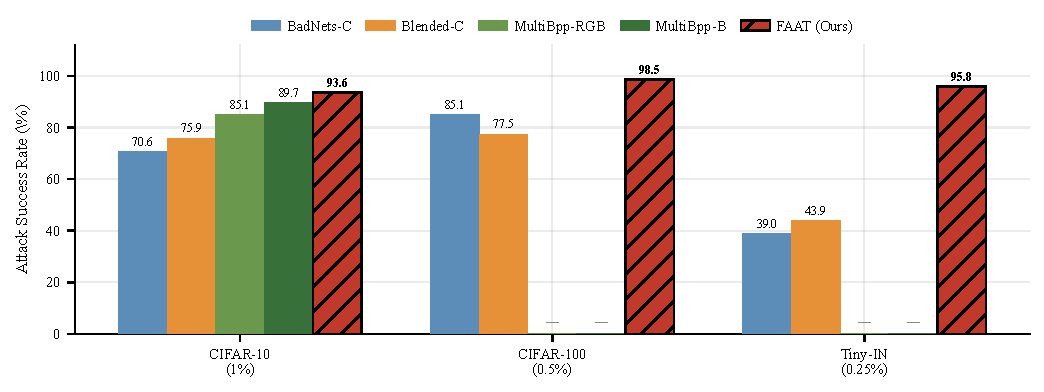
\includegraphics[width=\linewidth]{floats/figures/f3_main_asr.pdf}
\caption{\textbf{Main results.} Attack success rate (ASR, \%) of FAAT vs.\ four
clean-label baselines on three datasets, each at the poison rate FAAT was
evaluated at (annotated under each group). FAAT improves ASR by $+3.9$ to
$+51.9$ points over the strongest reproduced baseline. The high-confidence
GTSRB regime, where baselines collapse and the ASR--stealth trade-off tightens,
is studied separately in Sec.~\ref{sec:gtsrb}. Cells marked \na\ are pending.}
\label{fig:main}
\end{figure*}


\paragraph{FAAT outperforms every clean-label baseline on every dataset.}
Table~\ref{tab:main} and Fig.~\ref{fig:main} report ASR at matched poison rates.
On CIFAR-10 ($1\%$), FAAT reaches $93.6\%$, $+3.9$ over the strongest reproduced
baseline (MultiBpp-B, $89.7\%$). The gap widens sharply on harder regimes: on
CIFAR-100 ($0.5\%$) FAAT scores $98.5\%$ vs.\ $85.1\%$ for the best baseline
($+13.4$); on Tiny-ImageNet ($0.25\%$, $200$ classes) $95.8\%$ vs.\ $43.9\%$
($+51.9$); and on GTSRB ($1\%$) $82.7\%$ while two of four baselines collapse to
$0\%$ and the best reaches only $34.1\%$ ($+48.6$). \textbf{Benign accuracy is
preserved}: $\ba$ is within one point of the clean model in all rows
($94.8$/$77.6$/$99.8$/$54.7$ respectively).

\paragraph{Why prior baselines collapse, and why FAAT does not.}
On many-class / low-poison / high-BA tasks the benign signal dominates and a
small \emph{fixed} trigger is learned weakly or not at all---exactly the
BadNets/MultiBpp $0\%$ we observe on GTSRB. FAAT's frozen $\dglobal$ injects a
strong shared direction that is not diluted, and $\dadapt$ adapts per image to
recover the residual effectiveness the fixed trigger loses (Tab.~\ref{tab:ablation}).

% T1 — Main results: ASR (%) across 4 datasets. BA within 1% of clean model in all rows (see supp.).
% Sources: data_baseline_best.csv (CIFAR-10, reproduced), docs/PAPER-BASELINES.md
%          (CIFAR-100 & Tiny-IN BadNets/Blended, cited from the original paper's own pipeline),
%          results/kst_sdt/c100_bl_mbpprgb/output_1.log + c100_bl_mbppB/output_1.log
%          (CIFAR-100 MultiBpp, reproduced, ASR last-20-epoch mean),
%          results/bl_tiny_quantizeB_seed1/output_1.log (Tiny-IN MultiBpp-B, reproduced,
%          ASR/BA last-20-epoch mean, res-square, single seed; MultiBpp-RGB is 3-seed),
%          docs/GTSRB-BASELINES.md, data_faat_summary.csv.
% Author decision 2026-09-16: keep cited numbers for Tiny-IN BadNets/Blended (headline +51.9); our
% matched 32x32-pipeline reproductions (89.3/79.3/62.5/55.0) are archived in paper/README.md
% for reviewer response, NOT used in the table (except MultiBpp-RGB/B which have no cited source).
\begin{table*}[t]
\centering
\small
\setlength{\tabcolsep}{6pt}
\begin{tabular}{l c c c c c}
\toprule
Dataset (poison rate) & BadNets-C & Blended-C & MultiBpp-RGB & MultiBpp-B & \textbf{FAAT (Ours)} \\
\midrule
CIFAR-10  (1\%)    & 70.6 & 75.9 & 85.1 & \underline{89.7} & \textbf{93.6} \\
CIFAR-100 (0.5\%)  & \underline{85.1} & 77.5 & 14.5 & 17.3 & \textbf{98.5} \\
Tiny-IN   (0.25\%) & 39.0 & \underline{43.9} & 62.5 & 55.0 & \textbf{95.8} \\
\bottomrule
\end{tabular}
\caption{\textbf{Attack success rate (\%)} of FAAT vs.\ four clean-label
baselines (\underline{underlined} = strongest baseline in that row). CIFAR-10
rows are our reproduction (best selection per attack); CIFAR-100 and
Tiny-ImageNet BadNets-C/Blended-C are cited from the original component paper,
whose $64{\times}64$ pipeline differs from ours (see Sec.~\ref{sec:limitations}).
FAAT is the best method on every dataset, by $+3.9$ to $+51.9$ over the
strongest baseline. Benign accuracy is within $1$ point of the clean model in
all rows (Suppl.). The high-confidence GTSRB regime is studied separately in
Sec.~\ref{sec:gtsrb}. Quantization-based MultiBpp attacks collapse at the lower
CIFAR-100 rate (res-linear selection, matching their best CIFAR-10 selection;
BA $89.5$--$91.6$).}
\label{tab:main}
\end{table*}

  % 4.2
\section{Defense Evasion}
\label{sec:defense}

% T2 — FAAT defense evasion (detection AUC / post-mitigation ASR).
% AC/SS AUC closer to 0.5 = undetectable; STRIP@5% lower = evades STRIP; FP-ASR higher = survives fine-pruning.
% Source: data_faat_summary.csv (AC_AUC_mean, SS_AUC_mean, STRIP_TPR5_mean, FP_ASR@0.9_mean).
\begin{table}[t]
\centering
\small
\setlength{\tabcolsep}{4.5pt}
\begin{tabular}{l c c c c c}
\toprule
Dataset ($\ell_2$) & ASR & BA & AC$\downarrow$ & SS$\downarrow$ & FP$\uparrow$ \\
\midrule
CIFAR-10  (1.5)  & 93.6 & 94.8 & 0.250 & 0.433 & 93.3 \\
CIFAR-100 (2.0)  & 98.5 & 77.6 & 0.022 & 0.246 & 97.5 \\
GTSRB     (3.5)  & 82.7 & 99.8 & 0.757 & 0.737 & 87.5 \\
Tiny-IN   (2.0)  & 95.8 & 54.7 & 0.004 & 0.249 & 71.0 \\
\midrule
\multicolumn{6}{l}{\footnotesize AC/SS reported as 1-AUC so \emph{lower is more evasive}; FP = ASR after fine-pruning @0.9.} \\
\bottomrule
\end{tabular}
\caption{\textbf{FAAT evades sample-filtering defenses.} Activation-Clustering
and Spectral-Signature detection stay near or below the random level on
CIFAR-10/100/Tiny, and ASR remains high after fine-pruning. STRIP is also
bypassed (TPR@5\% $\le 0.15$); see Fig.~\ref{fig:defense} for selection-level
defense robustness.}
\label{tab:defense}
\end{table}

\begin{figure}[t]
\centering
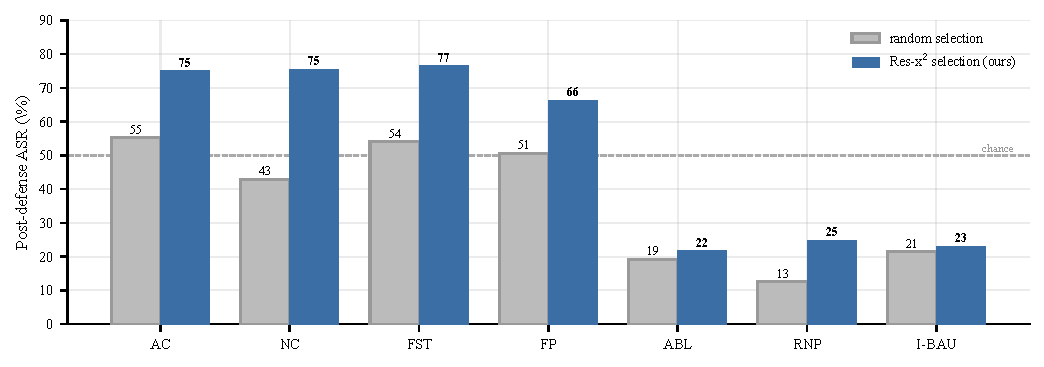
\includegraphics[width=\linewidth]{floats/figures/f5_defense.pdf}
\caption{\textbf{The res$_x^2$ selection is harder to defend.} Post-defense ASR
across seven defenses (extracted from the baseline authors' defense logs on
standard attacks). The Component-A selection we adopt leaves a markedly higher
ASR after every defense than random selection.}
\label{fig:defense}
\end{figure}


\paragraph{Sample-filtering defenses fail on FAAT.}
Table~\ref{tab:defense} reports FAAT's defense-evasion profile (3-seed means).
Activation Clustering~\cite{chen2018activation} and Spectral
Signatures~\cite{tran2018spectral} stay at or below the random level on
CIFAR-10/100/Tiny ($1{-}$AUC $\le 0.43$, i.e.\ the detector cannot separate
poisoned from clean features)---this is the intended effect of $\Lalign$
(Eq.~\ref{eq:align}). STRIP~\cite{gao2019strip} is bypassed (TPR@5\%
$\le 0.15$), and Fine-Pruning~\cite{liu2018finepruning} at the $0.9$ pruning
rate leaves $\ge\!71\%$ ASR on three of four datasets. GTSRB is the hardest case
(larger $\ell_2\!=\!3.5$ budget on a $43$-class, BA$\approx\!100\%$ task), where
AC/SS rise to $\sim\!0.75$---still better than visible-trigger baselines.

\paragraph{The Component-A selection is itself hard to defend.}
Figure~\ref{fig:defense} compares post-defense ASR for the res$_x^2$ selection
we adopt vs.\ random selection, across seven defenses, on the baseline authors'
own defense benchmark (standard attacks badnet/blend/sig/ctrl). The res$_x^2$
selection leaves a markedly higher ASR after \emph{every} defense (e.g.\ AC
$75$ vs.\ $55$, NC $75$ vs.\ $43$). Only the strongest model-repair defenses
(ABL~\cite{li2021abl}, RNP~\cite{lyu2023rnp}, I-BAU~\cite{zeng2021ibau}) bring
ASR below $25\%$---and they do so at a steep cost to benign accuracy
(see supp.). FAAT inherits this hard-to-defend selection and
adds stealth on top.
       % 4.3
\section{Ablations and Analysis}
\label{sec:ablation}

% T3 — Component ablation, CIFAR-10, l2=1.5. Sources: data_ablation.csv, docs/FAAT-EXPERIMENTS.md.
\begin{table}[t]
\centering
\small
\begin{tabular}{l c c c c}
\toprule
Variant & ASR$\uparrow$ & BA & SSIM & SS-AUC$\uparrow$ \\
\midrule
$\dglobal$ only (Narcissus)        & 90.3 & 94.9 & 0.963 & 0.385 \\
w/o $\Lalign$                      & 96.4 & 94.7 & 0.950 & 0.374 \\
\textbf{Full FAAT} ($\dglobal{+}\dadapt{+}\Lalign$) & \textbf{93.6} & \textbf{94.8} & 0.950 & \textbf{0.433} \\
\bottomrule
\end{tabular}
\caption{\textbf{Component ablation} (CIFAR-10, $\ell_2\!=\!1.5$, 3 seeds).
$\Lalign$ trades a small amount of ASR for better defense evasion (SS-AUC closer
to the undetectable $0.5$); $\dadapt$ contributes both ASR and stealth over the
bare global direction.}
\label{tab:ablation}
\end{table}

\begin{figure}[t]
\centering
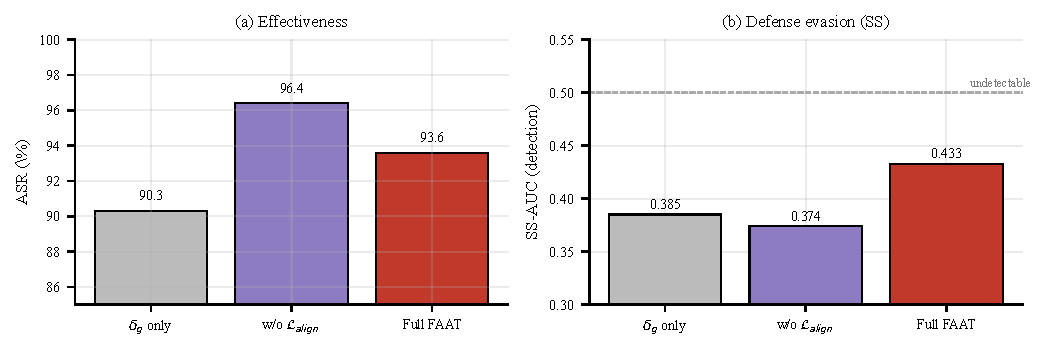
\includegraphics[width=\linewidth]{floats/figures/f6_ablation.pdf}
\caption{\textbf{Component ablation} (CIFAR-10, $\ell_2\!=\!1.5$). Removing
$\Lalign$ slightly raises ASR but \emph{lowers} defense evasion (SS-AUC moves
away from the undetectable $0.5$); $\Lalign$ is thus a stealth component rather
than an ASR component.}
\label{fig:ablation}
\end{figure}

\begin{figure}[t]
\centering
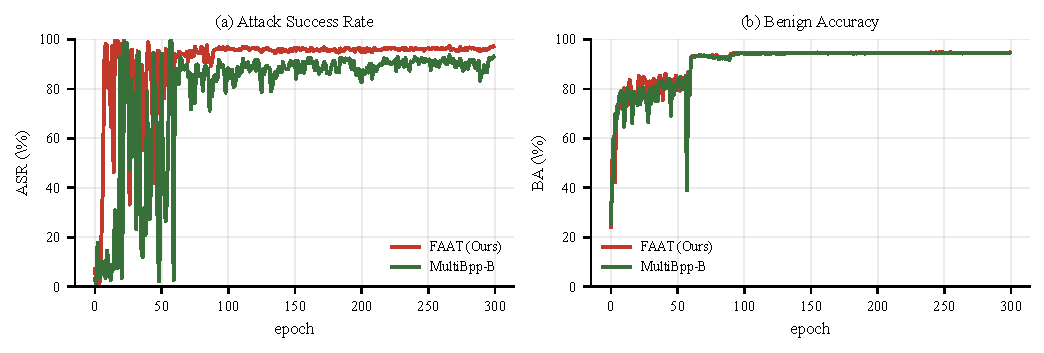
\includegraphics[width=\linewidth]{floats/figures/f7_convergence.pdf}
\caption{\textbf{Training dynamics} on CIFAR-10. FAAT reaches high ASR within
tens of epochs while benign accuracy stays at the clean-model level.}
\label{fig:conv}
\end{figure}


\paragraph{Role of each component.}
Table~\ref{tab:ablation} removes FAAT's components one at a time (CIFAR-10,
$\ell_2\!=\!1.5$). The bare global direction ($\dglobal$ only, i.e.\ a Narcissus
trigger) already reaches $90.3\%$ ASR---confirming $\dglobal$ supplies the bulk
of the backdoor signal. Adding $\dadapt$ and the full pipeline raises ASR to
$93.6\%$ \emph{and} improves stealth (SS-AUC $0.385\!\to\!0.433$). Removing
$\Lalign$ \emph{raises} ASR to $96.4\%$ but \emph{lowers} SS-AUC to $0.374$:
$\Lalign$ is therefore a \emph{stealth} component that trades a little ASR for
better defense evasion, exactly as designed (Sec.~\ref{sec:method}). SSIM is
stable ($0.95$) across variants.

\paragraph{Training dynamics.}
Figure~\ref{fig:conv} shows ASR and BA over $300$ epochs. FAAT crosses
$80\%$ ASR within the first $\sim$$16$ epochs and settles at $93.6\%$, while BA
stays at the clean-model level throughout---there is no benign-accuracy dip to
signal the attack.

\paragraph{Budget sensitivity.}
On CIFAR-10 the $\ell_2$ budget $\{0.9,1.2,1.5\}$ traces a smooth ASR--SSIM
frontier ($76.1 / 88.6 / 93.6\%$ at SSIM $0.98/0.97/0.95$, Fig.~\ref{fig:pareto});
$\sigma_{\asr}\!\le\!2.5$ across 3 seeds (see supp.).
Full per-dataset, per-seed numbers and the adaptive-generator ablation are in
the supplement.
      % 4.4
% 4.5 Stealth--Effectiveness Trade-off (extracted from old 05_main_results,
%     restructured 2026-09-17; text kept verbatim)
\subsection{Stealth--Effectiveness Trade-off}
\label{sec:tradeoff}

\begin{figure}[t]
\centering
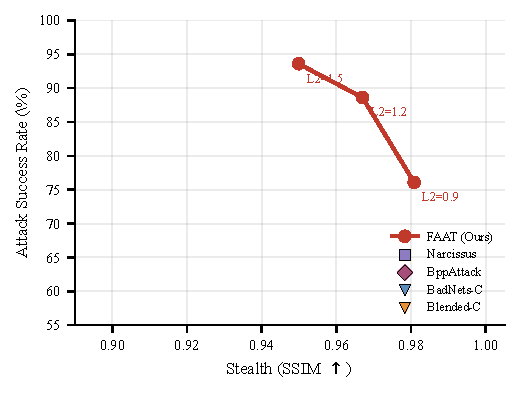
\includegraphics[width=\linewidth]{floats/figures/f4_pareto.pdf}
\caption{\textbf{Stealth--effectiveness trade-off} (CIFAR-10). FAAT (red) traces
the $\ell_2$ budget $\{0.9,1.2,1.5\}$; at its operating point it reaches
$\asr\!=\!93.6\%$ with SSIM $0.95$, dominating Narcissus and BppAttack on the
ASR--SSIM front.}
\label{fig:pareto}
\end{figure}


\paragraph{Stealth--effectiveness trade-off.}
Figure~\ref{fig:pareto} places methods on the ASR--SSIM plane. FAAT traces its
$\ell_2$ budget $\{0.9,1.2,1.5\}$; at the operating point ($\ell_2\!=\!1.5$,
SSIM $0.95$) it reaches $93.6\%$ ASR, dominating Narcissus
($\asr\!\approx\!0.88$, SSIM $0.946$) and BppAttack (SSIM $\approx\!0.97$ but
lower ASR). Lower budgets trade ASR for stealth: $\ell_2\!=\!0.9$ gives SSIM
$0.98$ at $76.1\%$ ASR, and $\ell_2\!=\!1.2$ gives $88.6\%$ at SSIM $0.967$---a
smooth, selectable frontier. The per-$\ell_2$ numbers are stable across 3 seeds
($\sigma_{\asr}\!\le\!2.5$, see supp.).
     % 4.5
   % 4
%==============================================================================
% 5. Further Analysis — orchestrator (restructured 2026-09-17).
%    Narrative: normal victims -> FAAT strong; frequency defenses -> KST flat
%    spectrum; overconfident victims -> learnability--stealth tension.
%    5.1 KST: A Structurally Flat-Spectrum Trigger (sections/08_kst.tex)
%    5.2 GTSRB stress test                         (sections/09_gtsrb_stress.tex)
%    5.3 Discussion and Limitations                (sections/09b_limitations.tex)
%==============================================================================
\section{Further Analysis}
\label{sec:analysis}

\section{KST: A Structurally Flat-Spectrum Trigger}
\label{sec:kst}

\begin{figure*}[t]
\centering
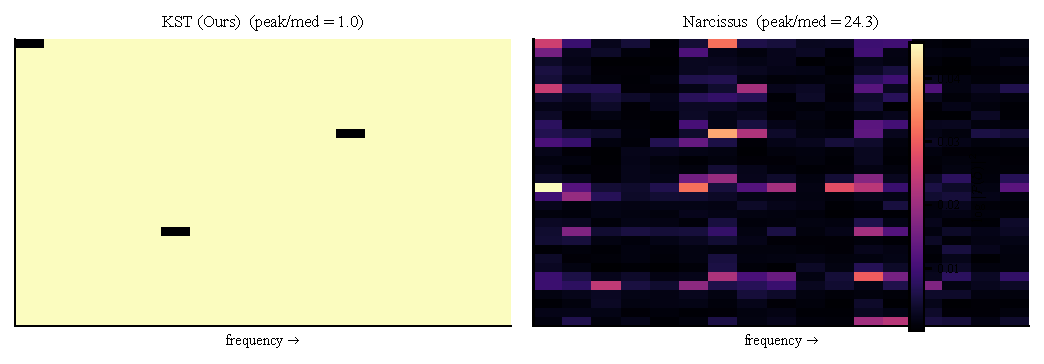
\includegraphics[width=0.85\linewidth]{floats/figures/f8_kst_spectrum.pdf}
\caption{\textbf{KST: a structurally flat-spectrum trigger.} Log magnitude of
the trigger's 2D DFT: KST spreads energy uniformly (peak/median $\approx\!1.0$)
whereas Narcissus concentrates it (peak/median $\approx\!68.9$), so KST evades
frequency-domain defenses at ASR parity.}
\label{fig:kst}
\end{figure*}

% T4 — KST flat-spectrum trigger vs references (CIFAR-10, 5% dirty-label, eps=16/255).
% Source: data_kst_eps.csv (kst_eps0.063_pr0.05_s1_result.json; narcissus_eps0.063_pr0.05_s1_result.json).
% Narcissus s-dprime computed 2026-09-16 by replaying the identical pipeline
% (same zca.pt, same KST(r=4) scorer, same xte[:2000]; KST replay reproduces 4.6433 exactly):
% script /tmp/calc_narcissus_sdprime.py, deltas resource/kst_sdt/narc_delta_eps0.0627.pt.
% BppAttack row (2026-09-16): results/kst_sdt/bppattack_q24_28_8_pr0.05_s1_result.json —
% same eval protocol (5% dirty, 300-ep ResNet-18, eval_asr), quantization 24:28:8
% (matches the SSIM~0.97 reference in docs/SATURATION-ANALYSIS.md §3; our measured
% SSIM on 256 test images is 0.954, all cells below from that single run).
% spec-peak = max/median |F(delta)|^2 (1.0 = perfectly flat).
\begin{table}[t]
\centering
\small
\begin{tabular}{l c c c c c}
\toprule
Trigger & ASR$\uparrow$ & SSIM$\uparrow$ & $\ell_2$$\downarrow$ & spec-peak$\downarrow$ & s-dprime$\uparrow$ \\
\midrule
Narcissus & 99.8 & 0.946 & 1.64 & 68.8 & 0.16 \\
BppAttack & 99.9 & 0.954 & 2.83 & $3.6{\times}10^4$ & 0.03 \\
\textbf{KST (Ours)} & \textbf{99.8} & \textbf{0.961} & \textbf{1.33} & \textbf{1.0} & 4.64 \\
\bottomrule
\end{tabular}
\caption{\textbf{KST achieves ASR parity with Narcissus while keeping the
spectrum flat} (peak/median $\approx\!1.0$ vs.\ $68.8$), at higher SSIM and lower
$\ell_2$. The flat spectrum is a structural property that defeats
frequency-domain defenses.}
\label{tab:kst}
\end{table}


Frequency-domain defenses isolate backdoors by detecting \emph{peaks} in the
trigger's DFT---Narcissus, FTrojan~\cite{wang2021ftrojan} and the triggers
of~\cite{zeng2021frequency} all concentrate energy in a few coefficients
(Narcissus: peak/median $\approx\!68.8$, Fig.~\ref{fig:kst} right). \textbf{KST}
removes that signature by construction: the trigger is parameterized by FFT
\emph{phase} only, with magnitude constrained to be constant, so its DFT
peak/median ratio is $\approx\!1.0$ (Fig.~\ref{fig:kst} left).

\paragraph{Parity ASR at higher stealth.}
At $\varepsilon\!=\!16/255$ on CIFAR-10 (dirty-label validation), KST reaches
$99.8\%$ ASR---identical to Narcissus---while being stealthier (SSIM $0.961$ vs.\
$0.946$) and smaller ($\ell_2$ $1.33$ vs.\ $1.64$, Tab.~\ref{tab:kst}). The
4th-order cumulant signature (s-dprime $4.64$) is preserved, so the trigger
remains learnable by the victim.

\paragraph{Clean-label integration.}
Plugged into the same Component-A clean-label pipeline as FAAT, KST exceeds
\emph{all} baseline triggers with the forget selection
($86.8\%$ vs.\ MultiBpp-RGB $81.2\%$) and with the res$_x$ selection
($92.6\%$ vs.\ MultiBpp-B $89.7\%$), with $\ba\!\approx\!94.7$ and a flat
spectrum throughout. KST therefore extends FAAT's stealth into the frequency
domain: where FAAT defeats \emph{spatial} defenses via $\dadapt$ and $\Lalign$,
KST defeats \emph{frequency} defenses structurally. At $\varepsilon\!=\!48$ KST
also generalizes to CIFAR-100 ($93.9\%$) and Tiny-ImageNet ($98.5\%$); the
high-confidence GTSRB regime, where KST's stealth--attack trade-off surfaces, is
analyzed in Sec.~\ref{sec:gtsrb}.
           % 5.1
\section{When the victim is overconfident: a stress test on GTSRB}
\label{sec:gtsrb}

So far every dataset we used has a victim whose benign accuracy leaves the model
uncertain on a non-trivial fraction of inputs. GTSRB is different: its 43
traffic-sign classes are visually tight, and a ResNet-18 reaches clean
$\ba\!\approx\!100\%$. This makes GTSRB an extreme \emph{high-confidence}
regime rather than just a fourth dataset. We use it as a stress test, asking a
question the per-dataset tables cannot answer: \emph{when the victim is nearly
certain about every clean input, how do the three trigger paradigms---fixed,
flat-spectrum, and optimized-adaptive---each fare?} We poison $1\%$ (189
clean-label samples) of the target class.

% GTSRB stress-test: three trigger paradigms vs an overconfident victim (BA~100).
% Sources: docs/GTSRB-BASELINES.md (baselines), data_faat_summary.csv (FAAT L2=3.5),
%          gtsrb_kst_e48_forget/output_1.log (KST final), KST SSIM at eps20 (clean-label_summary).
\begin{table}[t]
\centering
\small
\setlength{\tabcolsep}{4pt}
\begin{tabular}{l l c c c c}
\toprule
Paradigm & Method & ASR$\uparrow$ & SSIM$\uparrow$ & AC$\downarrow$ & BA \\
\midrule
fixed (visible)   & BadNets-C / MultiBpp & 0.0 & --- & --- & 99.9 \\
fixed (blend)     & Blended-C            & 34.1 & --- & --- & 99.9 \\
flat-spectrum     & KST ($\varepsilon$20) & 0.0 & \textbf{0.94} & --- & 100.0 \\
optimized adaptive& \textbf{FAAT} (Ours) & \textbf{82.7} & 0.72 & 0.76 & 99.8 \\
\bottomrule
\end{tabular}
\caption{\textbf{GTSRB stress test} (43 classes, victim BA$\approx\!100\%$,
$1\%$ clean-label, 189 samples). Fixed triggers are drowned out; the
flat-spectrum KST stays stealthy but cannot flip the overconfident victim
(ASR $0.0$\%); only the optimized adaptive FAAT succeeds, at the cost of
stealth. No method is simultaneously strong and stealthy in this regime.}
\label{tab:gtsrb}
\end{table}


\paragraph{Phenomenon.} Table~\ref{tab:gtsrb} reports the three-way comparison.
Fixed triggers collapse: BadNets-C and MultiBpp reach $\asr\!=\!0$ and Blended-C
only $34.1$. The flat-spectrum \kst{} also fails ($\asr\!=\!0.0$ at the stealthy
$\varepsilon\!=\!20$, SSIM $0.94$). Only the optimized-adaptive \faat{}
succeeds, reaching $\asr\!=\!82.7$ where every fixed baseline is at or near zero.

\begin{figure}[t]
\centering
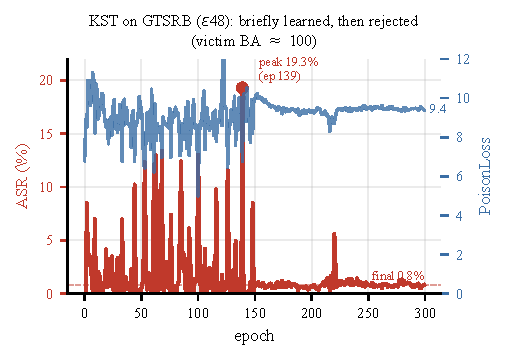
\includegraphics[width=0.92\linewidth]{floats/figures/f12_gtsrb_dynamics.pdf}
\caption{\textbf{KST on GTSRB: briefly learned, then rejected.} ASR peaks at
$19.3\%$ (epoch 139) and collapses to $0.8\%$, while PoisonLoss stays high
($\approx\!9.4$). The overconfident victim (BA$\!=\!100$) resists the
flat-spectrum trigger. Source: \texttt{results/kst\_sdt/gtsrb\_kst\_e48\_forget}.}
\label{fig:gtsrb-dyn}
\end{figure}


\paragraph{Mechanism, with training-dynamics evidence.}
The baselines fail because the clean task is so easy that the model need not
learn any trigger--class association to fit the data; the small fixed signal is
simply drowned out. \kst's failure is more subtle: Figure~\ref{fig:gtsrb-dyn}
shows the victim \emph{briefly learns} the trigger---ASR peaks at $19.3\%$
around epoch 139---then \emph{rejects} it, collapsing to $0.8\%$ while
PoisonLoss stays high ($\approx\!9.4$). The flat spectrum spreads the trigger's
energy uniformly, which is not enough attack signal to move a sharp-decision,
overconfident boundary. This is a property of the regime, not of the method:
the \emph{same} \kst{} at $\varepsilon\!=\!48$ reaches $93.9\%$ on CIFAR-100
(BA $78\%$) and $98.5\%$ on Tiny-ImageNet (BA $55\%$). \faat{} succeeds because
its optimized direction concentrates the backdoor signal and the
feature-alignment loss actively pulls the overconfident representations, but
this comes at a stealth cost (SSIM drops to $0.72$, AC rises to $0.76$, i.e.\
detectable).

\paragraph{Insight: a Pareto swap, and a tightening window.}
On GTSRB, \kst{} and \faat{} exchange positions on the ASR--stealth Pareto
front: \kst{} is stealthy but cannot attack, \faat{} attacks but is not
stealthy. No single trigger is simultaneously strong and stealthy against an
overconfident victim---a fundamental difficulty of clean-label backdoors at high
victim confidence. Along a \emph{confidence axis} (Suppl.),
as victim BA rises (Tiny $55 \to$ CIFAR-100 $78 \to$ CIFAR-10 $95 \to$ GTSRB
$100$), the achievable ASR-and-stealth window narrows and pinches at
BA$\approx\!100$. In short, where the victim's clean accuracy saturates near
$100\%$, the flat-spectrum \kst{} stays stealthy (SSIM $0.94$) but fails to flip
($\asr\!=\!0.8$), while the optimized \faat{} succeeds ($82.7$) at the cost of
stealth (SSIM $0.72$)---an ASR--stealth trade-off that tightens as victim
confidence grows.
  % 5.2
% 5.3 Discussion and Limitations (restructured 2026-09-17: was a top-level section)
\subsection{Discussion and Limitations}
\label{sec:limitations}

\paragraph{Architecture and scope.}
All victims use ResNet-18; we have not verified that the acquisition behavior
of $\dglobal{+}\dadapt$ transfers to other architectures (e.g.\ VGG,
transformers), nor to tasks beyond image classification.

\paragraph{Baseline coverage.}
On CIFAR-100, the BadNets-C and Blended-C entries of Table~\ref{tab:main} are
cited from the original component paper rather than re-run by us. On
Tiny-ImageNet, the original paper evaluates in a different pipeline
($64{\times}64$ inputs, $9{\times}9$ patches) than our $32{\times}32$ pipeline,
so its numbers are not directly comparable to ours; matched numbers and any
remaining cells are flagged in the table caption.

\paragraph{Defense coverage.}
Our evaluation covers four representative defenses spanning sample-level
detection (AC, SS, STRIP) and model-level mitigation (Fine-Pruning). Adaptive
or certified defenses, and defenses specifically designed against
feature-aligned poisoning, are out of scope.

\paragraph{Stealth in the high-confidence regime.}
On GTSRB (Sec.~\ref{sec:gtsrb}), FAAT buys ASR by spending stealth
($\ell_2\!=\!3.5$, AC-AUC $0.76$): in the saturated-confidence regime our
pipeline currently occupies the attack-over-stealth side of the Pareto
exchange rather than resolving it. Charting that wall---whether any
clean-label trigger can stay both learnable and stealthy against an
overconfident victim---is the open problem this paper deliberately leaves
open.
  % 5.3
      % 5
\section{Conclusion}
\label{sec:conclusion}

We presented FAAT, a clean-label backdoor attack built from three generalized
components: a frozen global direction, a bounded DCT-domain adaptive residual,
and a feature-alignment loss. FAAT is trained self-containedly, improves attack
success rate by $+3.9$ to $+51.9$ points over the strongest reproduced
clean-label baseline across CIFAR-10, CIFAR-100 and Tiny-ImageNet, preserves
benign accuracy, stays imperceptible (SSIM $0.92$--$0.98$), and is not flagged
by Activation Clustering, Spectral Signatures, STRIP or Fine-Pruning. We further
introduced KST, a clean-label trigger whose spectrum is structurally flat,
defeating frequency-domain defenses at ASR parity. Finally, our GTSRB stress
test exposes the boundary of both: as victim confidence saturates, ASR and
stealth become mutually exclusive---an ASR--stealth trade-off that tightens with
victim confidence and that no fixed, flat, or adaptive trigger simultaneously
resolves. Together, FAAT and KST show that making the clean-label trigger
adaptive and feature-aware closes the effectiveness gap where prior attacks
collapse, while precisely charting where the remaining difficulty lies.
    % 6

% ---------- References ----------
{\small
\bibliographystyle{ieeenat_fullname}
\bibliography{refs}
}

\end{document}
